\subsection{Эксперимент 1. Анализ оптимальных  параметров для GD.}
\subsubsection{Дизайн эксперимента}
В ходе данного эксперимента исследовались параметры для GD:
\begin{itemize}
	\item $\alpha$ - размер шага в \ref{step} (по логарифмической сетке)
	\item $\beta$ - размер шага в \ref{step} (по логарифмической сетке)
	\item $\omega_0$ - начальное приближение в \ref{grad}
\end{itemize}
В  данном эксперименте при выборе оптимального параметра остальные фиксировались. Выбор наилучшего параметра определялся из значений {\itshape accuracy} на валидационной выборке. При поиске следующих оптимальных параметров в качестве значений уже обработанных параметров брались найденные для них наилучшие параметры. Таким образом, в ходе эксперимента изучался не только вопрос устойчивой оптимальной сходимости функции потерь к минимуму, но также жадно подбирались наилучшие параметры, что в последующем будет использовано в последнем эксперименте. 
\subsubsection{Результаты эксперимента}
\begin{enumerate}
	\item {\bfseries  Выбор $\alpha$}
	
	Фиксируем $\beta = 1$ и $\omega_0 = 0 \in \mathbb{R}^D$ и по логарифмической сетке рассмотрим различные параметры $\alpha$ (см. рис.\ref{eq:exp1_fig1}).
    \newsavebox{\myimage}
    \begin{figure*}[h]
        \begin{subfigure}{.5\textwidth}
            \centering
            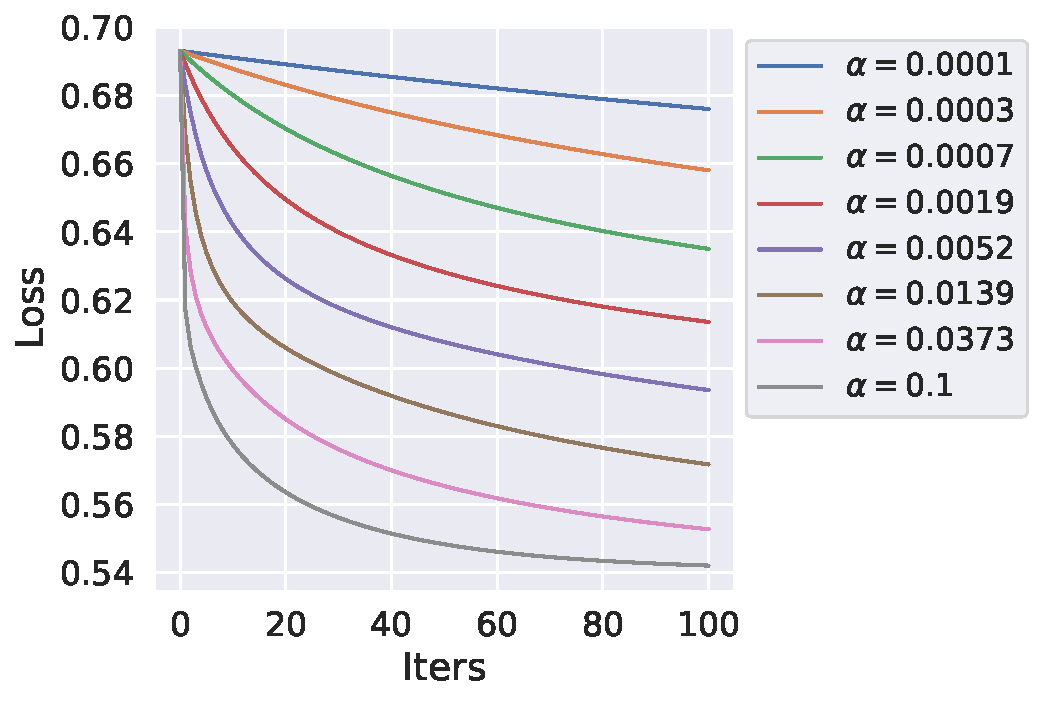
\includegraphics[width=\linewidth]{./experiment1/alpha/gd_loss__iters.pdf}
            \caption{}
        \end{subfigure}%
        \begin{subfigure}{.5\textwidth}
            \centering
            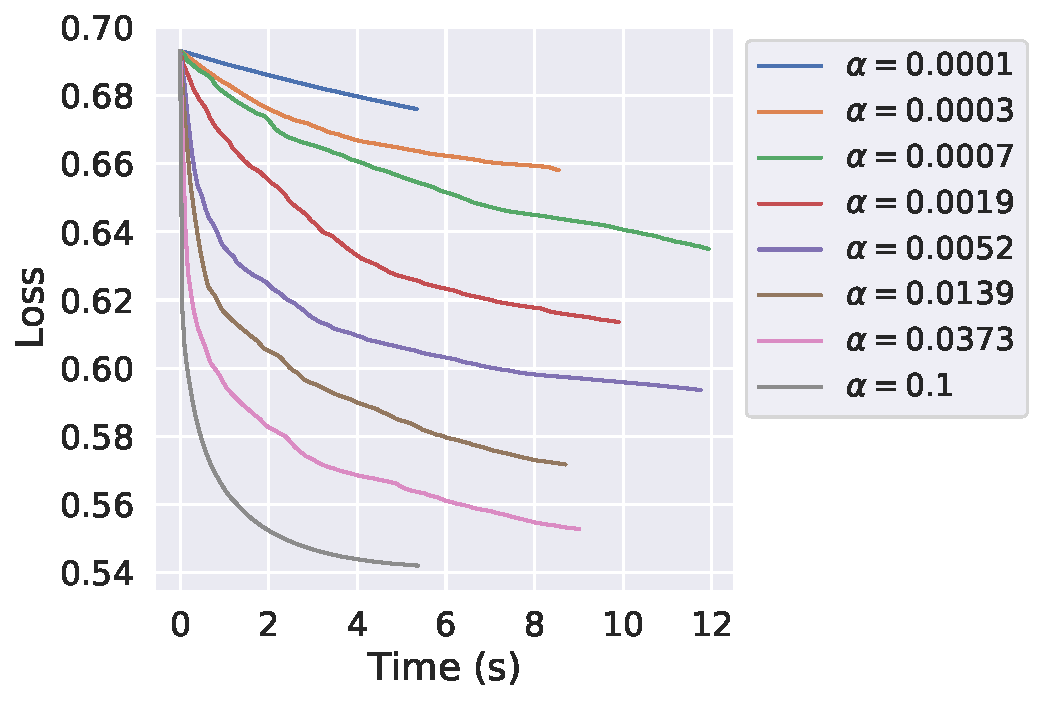
\includegraphics[width=\linewidth]{./experiment1/alpha/gd_loss_time.pdf}
            \caption{}
        \end{subfigure}
    \caption{}
	\end{figure*}\label{eq:exp1_fig1}
	Все графики зависимости от времени и итераций очень похожи друг на друга, поэтому в зависимости от потребностей в дальнейшем будут использоваться как графики от итераций так и графики от времени, а остальные будут помещены в {\bfseries Приложении А}. Из рис.\ref{eq:exp1_fig1} видно, что чем меньше $\alpha$ тем медленнее сходится к минимуму итерационный процесс, ему необходимо больше шагов итераций, так как темп обучения слишком мал. Впрочем, и слишком большие значения $\alpha$ не способствуют хорошей оптимизации (см. рис. \ref{eq:exp1_fig2}).
	\begin{figure}[h]
		
		\centering{
		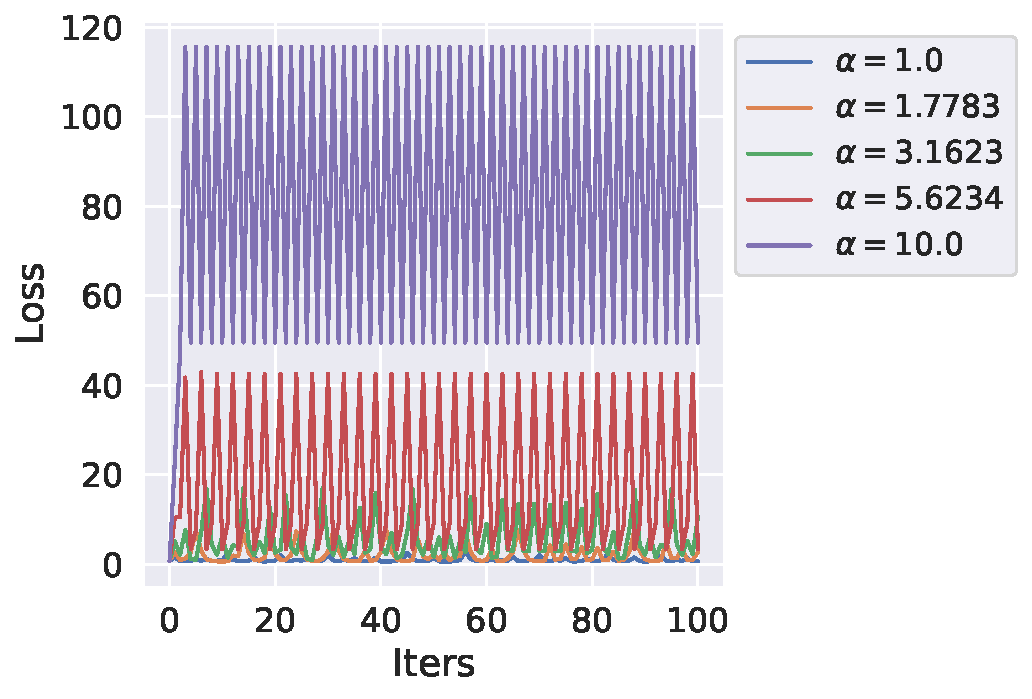
\includegraphics[width=0.8\textwidth]{./experiment1/alpha/gd_loss__iters_big_alphas.pdf}
		}
		\caption{}
		\label{eq:exp1_fig2}
	\end{figure}
	В результате выбора больших $\alpha \gtrapprox\!\!1.0$ уже наблюдается сильная осцилляция. При дальнейшем увеличение градиентный спуск на каждой итерации будет осциллировать около точки минимума(причем из графика видно, что при $\alpha = 10$ оцилляция уже происходит в области другой точки минимума). 
	Отрицательные значения  $\alpha$ бессмысленны, так как мы решаем задачу минимизации, а значит, нам нужен антиградиет, то есть градиент со знаком минус.
    %\newsavebox{\myimage}
    \begin{figure*}[h]
        \begin{subfigure}{.5\textwidth}
            \centering
            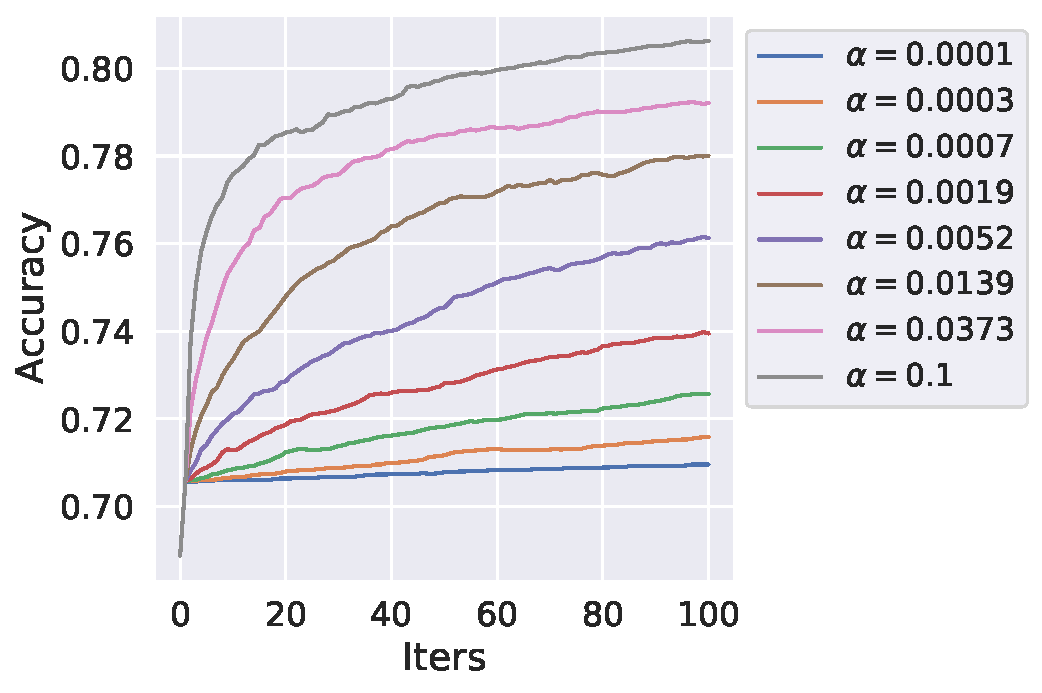
\includegraphics[width=\linewidth]{./experiment1/alpha/gd_acc_iters.pdf}
            \caption{}
        \end{subfigure}%
        \begin{subfigure}{.5\textwidth}
            \centering
            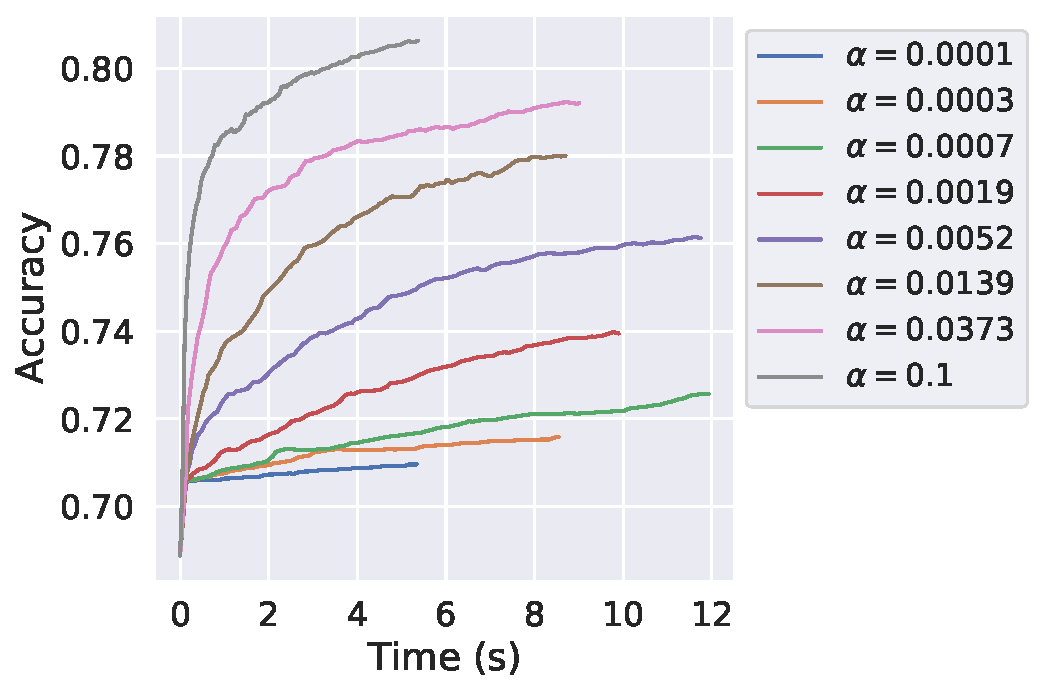
\includegraphics[width=\linewidth]{./experiment1/alpha/gd_acc_time.pdf}
            \caption{}
        \end{subfigure}
    \caption{}
    \label{eq:exp1_fig3}
	\end{figure*}
	Как видим из рис.\ref{eq:exp1_fig3} c увеличением $\alpha$ (при достаточно малых $\alpha$) быстрее достигается лучший accuracy. 
	
	\item{\bfseries  Выбор $\beta$}
	
	Теперь фиксируем $\alpha = 0.1$. При этом $\omega_0$ оставим той же. Будем перебирать по логарифмической сетке параметры $\beta$ 
    \begin{figure*}[h]
        \begin{subfigure}{.5\textwidth}
            \centering
            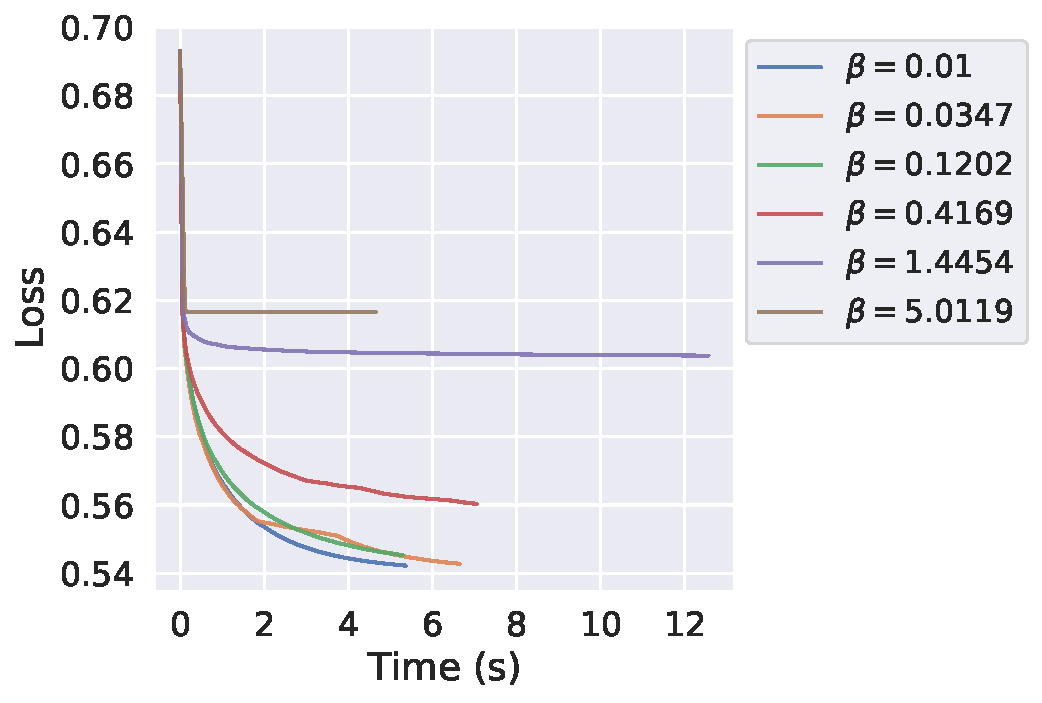
\includegraphics[width=\linewidth]{./experiment1/beta/gd_loss_time.pdf}
            \caption{}
        \end{subfigure}%
        \begin{subfigure}{.5\textwidth}
            \centering
            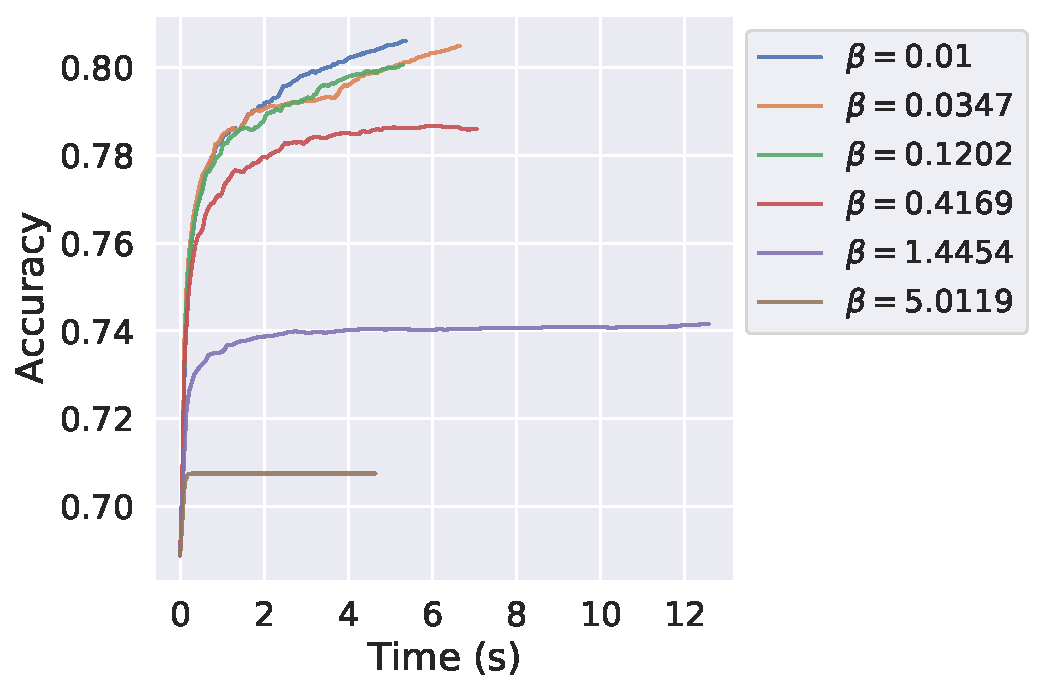
\includegraphics[width=\linewidth]{./experiment1/beta/gd_acc_time.pdf}
            \caption{}
        \end{subfigure}
    \caption{}
    \label{eq:exp1_fig4}
	\end{figure*}
	
	Из графика (рис.\ref{eq:exp1_fig4}) видно, что с уменьшением $\beta$ оптимизационная задача быстрее сходится к минимуму. При слишком больших $\beta\gtrapprox\!\!5$ алгоритм очень быстро закончит работать, поскольку из-за маленьких темпов обучения $\omega_k$(см. (\ref{grad})) будет не значительно меняться. С учетом гладкости функционала (см. Теоретическую часть) и его значения будут мало изменяться, следовательно условие останова цикла ($|Q(w_{k+1}) - Q(w_{k})| < tolerance$) будет быстро достигнуто и функция плохо решит оптимизационную задачу.

	Из рис.\ref{eq:exp1_fig4} следуют те же выводы, что и в случае с $\alpha$: c уменьшением $\beta$ оптимальная точность быстрее достигается

	\item{\bfseries  Выбор $\omega_0$}
	
	Фиксируем $\alpha = 0.1$, $\beta = 0.01$. Переберем $\omega_0$(см рис.\ref{eq:exp1_fig7}).
	\begin{figure}[h]		
		\centering{
		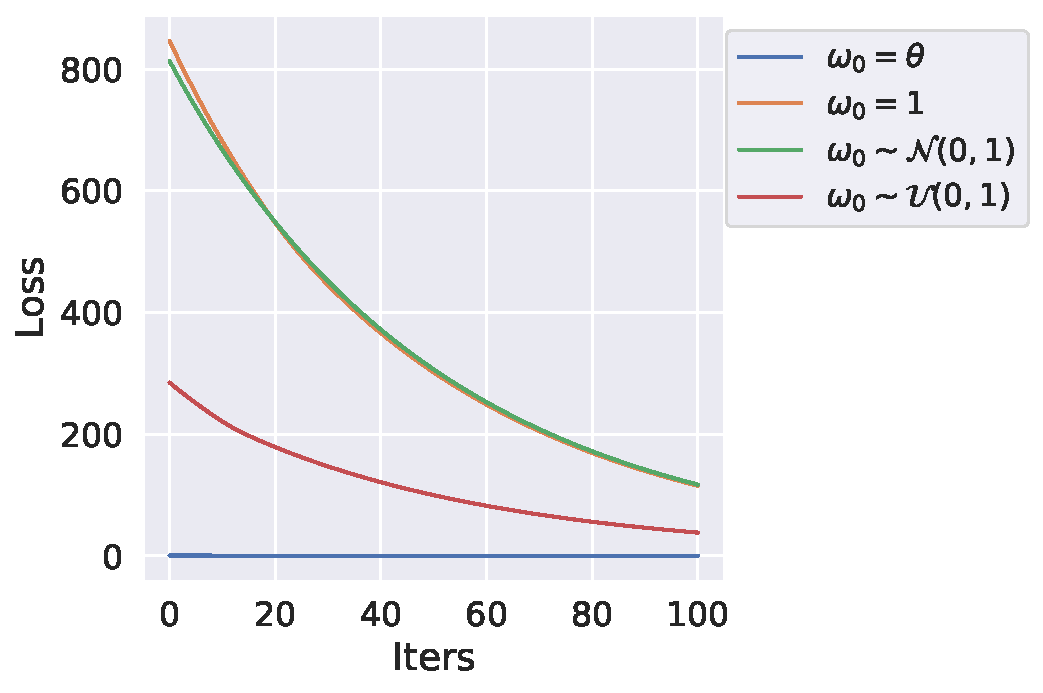
\includegraphics[width=0.8\textwidth]{./experiment1/w_0/gd_loss_iters.pdf}
		}
		\caption{}
		\label{eq:exp1_fig7}
	\end{figure}

	Некоторые пояснения:
	\begin{itemize}
		\item $\mathcal{N}$ - нормальное распределение
		\item $\mathcal{U}$ - равномерное распределение
	\end{itemize}
	Из графика (см. рис.\ref{eq:exp1_fig7}) видно, что с увеличением нормы $\omega_0$ значение функции потерь принимает большие значения. Лучшим вариантом будет взять $\omega_0 = 0$, тогда будет тратиться меньшее количество итераций на минимизацию, так как иначе сначала уйдет большое количество итераций на уменьшение больших значений функционала, а потом проблема возникнет с шагом (см. \ref{step}), так как он уже будет мал и значения функционала будут незначительно изменяться.\\
	Теперь посмотрим на точность при различных $\omega_0$ (см. рис. \ref{eq:exp1_fig8})
	\begin{figure}[h]		
		\centering{
		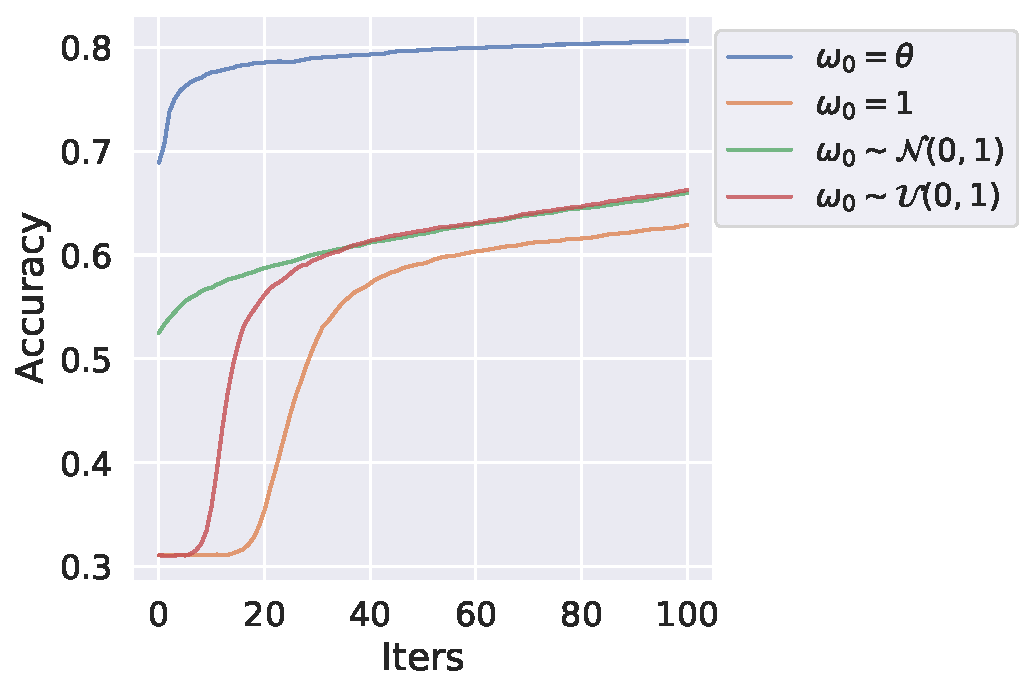
\includegraphics[width=0.8\textwidth]{./experiment1/w_0/gd_acc_iters.pdf}
		}
		\caption{}
		\label{eq:exp1_fig8}
	\end{figure}
\end{enumerate}
Точность также показывает правильность выбора начального приближения равного нулю.
\subsubsection{Выводы эксперимента}
Для градиентного спуска оптимальным будет следующий выбор параметров:
\begin{itemize}
	\item $\alpha \lessapprox\!1.0$
	\item $\beta \lessapprox\!0.15$
	\item $w = 0$, $0 \in \mathbb{R}^D$
\end{itemize}

